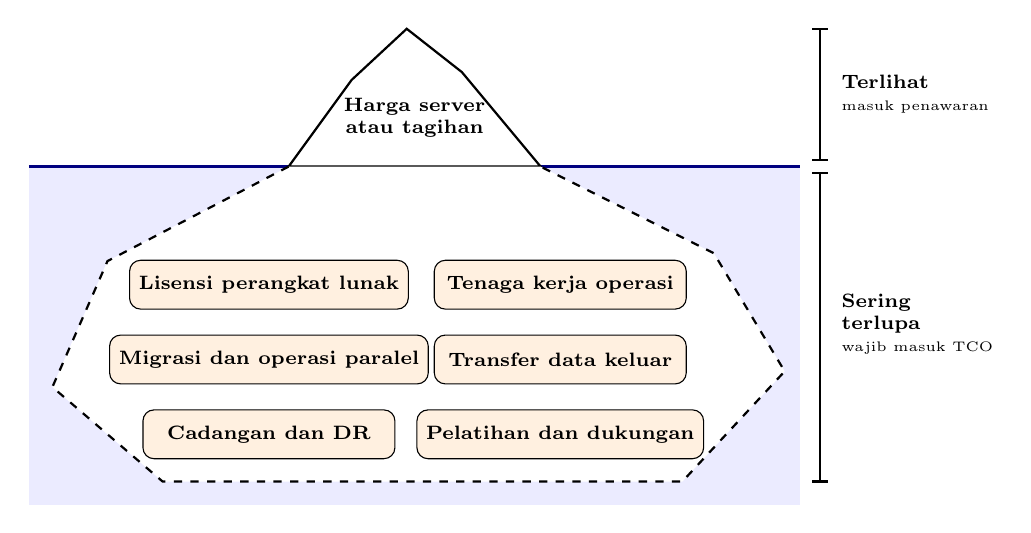
\begin{tikzpicture}[
  font=\scriptsize,
  panah/.style={-{Stealth[length=2mm]}, thick},
  biaya/.style={draw, rounded corners, fill=orange!12, minimum width=3.2cm,
    minimum height=0.62cm, align=center, font=\scriptsize\bfseries}
]
  % Permukaan air memisahkan biaya yang terlihat dan biaya yang sering terlupa.
  \fill[blue!8] (-4.9,-4.3) rectangle (4.9,0);
  \draw[thick, blue!50!black] (-4.9,0) -- (4.9,0);

  % Puncak gunung es: bagian yang muncul di penawaran harga.
  \draw[thick, fill=white] (-1.6,0) -- (-0.8,1.1) -- (-0.1,1.75) -- (0.6,1.2)
    -- (1.6,0) -- cycle;
  \node[font=\scriptsize\bfseries, align=center] at (0,0.62)
    {Harga server\\atau tagihan};

  % Badan gunung es di bawah air: komponen TCO yang sering terlupa.
  \draw[thick, dashed, fill=white] (-1.6,0) -- (-3.9,-1.2) -- (-4.6,-2.8)
    -- (-3.2,-4.0) -- (3.4,-4.0) -- (4.7,-2.6) -- (3.8,-1.1) -- (1.6,0);

  \node[biaya] at (-1.85,-1.5) {Lisensi perangkat lunak};
  \node[biaya] at (1.85,-1.5) {Tenaga kerja operasi};
  \node[biaya] at (-1.85,-2.45) {Migrasi dan operasi paralel};
  \node[biaya] at (1.85,-2.45) {Transfer data keluar};
  \node[biaya] at (-1.85,-3.4) {Cadangan dan DR};
  \node[biaya] at (1.85,-3.4) {Pelatihan dan dukungan};

  % Penanda kelompok di sisi kanan.
  \draw[thick] (5.15,1.75) -- (5.15,0.08);
  \draw[thick] (5.05,1.75) -- (5.25,1.75);
  \draw[thick] (5.05,0.08) -- (5.25,0.08);
  \node[anchor=west, align=left] at (5.3,0.92)
    {\textbf{Terlihat}\\{\tiny\mdseries masuk penawaran}};
  \draw[thick] (5.15,-0.08) -- (5.15,-4.0);
  \draw[thick] (5.05,-0.08) -- (5.25,-0.08);
  \draw[thick] (5.05,-4.0) -- (5.25,-4.0);
  \node[anchor=west, align=left] at (5.3,-2.0)
    {\textbf{Sering}\\\textbf{terlupa}\\{\tiny\mdseries wajib masuk TCO}};
\end{tikzpicture}
